% $Id: template.tex 11 2007-04-03 22:25:53Z jpeltier $

% 22 DEC 2023 added for accessibility tagging
% \DocumentMetadata{testphase=phase-III}
\documentclass{vgtc}                          % final (conference style)
% \documentclass[review]{vgtc}                 % review
%\documentclass[widereview]{vgtc}             % wide-spaced review
% \documentclass[preprint]{vgtc}               % preprint
%\documentclass[electronic]{vgtc}             % electronic version

%% Uncomment one of the lines above depending on where your paper is
%% in the conference process. ``review'' and ``widereview'' are for review
%% submission, ``preprint'' is for pre-publication, and the final version
%% doesn't use a specific qualifier. Further, ``electronic'' includes
%% hyperreferences for more convenient online viewing.

%% Please use one of the ``review'' options in combination with the
%% assigned online id (see below) ONLY if your paper uses a double blind
%% review process. Some conferences, like IEEE Vis and InfoVis, have NOT
%% in the past.

%% Figures should be in CMYK or Grey scale format, otherwise, colour 
%% shifting may occur during the printing process.

%% These few lines make a distinction between latex and pdflatex calls and they
%% bring in essential packages for graphics and font handling.
%% Note that due to the \DeclareGraphicsExtensions{} call it is no longer necessary
%% to provide the the path and extension of a graphics file:
%% \includegraphics{diamondrule} is completely sufficient.
%%
\ifpdf%                                % if we use pdflatex
  \pdfoutput=1\relax                   % create PDFs from pdfLaTeX
  \pdfcompresslevel=9                  % PDF Compression
  \pdfoptionpdfminorversion=7          % create PDF 1.7
  \ExecuteOptions{pdftex}
  \usepackage{graphicx}                % allow us to embed graphics files
  \DeclareGraphicsExtensions{.pdf,.png,.jpg,.jpeg} % for pdflatex we expect .pdf, .png, or .jpg files
\else%                                 % else we use pure latex
  \ExecuteOptions{dvips}
  \usepackage{graphicx}                % allow us to embed graphics files
  \DeclareGraphicsExtensions{.eps}     % for pure latex we expect eps files
\fi%

%% it is recomended to use ``\autoref{sec:bla}'' instead of ``Fig.~\ref{sec:bla}''
\graphicspath{{figures/}{pictures/}{images/}{./}} % where to search for the images

\usepackage{microtype}                 % use micro-typography (slightly more compact, better to read)
\PassOptionsToPackage{warn}{textcomp}  % to address font issues with \textrightarrow
\usepackage{textcomp}                  % use better special symbols
\usepackage{mathptmx}                  % use matching math font
\usepackage{times}                     % we use Times as the main font
\renewcommand*\ttdefault{txtt}         % a nicer typewriter font
\usepackage{cite}                      % needed to automatically sort the references
\usepackage{tabu}                      % only used for the table example
\usepackage{booktabs}                  % only used for the table example
%% We encourage the use of mathptmx for consistent usage of times font
%% throughout the proceedings. However, if you encounter conflicts
%% with other math-related packages, you may want to disable it.


%% If you are submitting a paper to a conference for review with a double
%% blind reviewing process, please replace the value ``0'' below with your
%% OnlineID. Otherwise, you may safely leave it at ``0''.
\onlineid{1007}

%% declare the category of your paper, only shown in review mode
\vgtccategory{Research}

%% allow for this line if you want the electronic option to work properly
\vgtcinsertpkg

%% In preprint mode you may define your own headline. If not, the default IEEE copyright message will appear in preprint mode.
%\preprinttext{To appear in an IEEE VGTC sponsored conference.}

%% This adds a link to the version of the paper on IEEEXplore
%% Uncomment this line when you produce a preprint version of the article 
%% after the article receives a DOI for the paper from IEEE
%\ieeedoi{xx.xxxx/TVCG.201x.xxxxxxx}


%% Paper title.

% \begin{document}

% \title{Global Illumination for Fun and Profit}
\title{Exposing Movement Correlates of Presence Experience in Virtual Reality using Parametric Maps}

%% This is how authors are specified in the conference style

%% Author and Affiliation (single author).
%%\author{Roy G. Biv\thanks{e-mail: roy.g.biv@aol.com}}
%%\affiliation{\scriptsize Allied Widgets Research}

%% Author and Affiliation (multiple authors with single affiliations).
%%\author{Roy G. Biv\thanks{e-mail: roy.g.biv@aol.com} %
%%\and Ed Grimley\thanks{e-mail:ed.grimley@aol.com} %
%%\and Martha Stewart\thanks{e-mail:martha.stewart@marthastewart.com}}
%%\affiliation{\scriptsize Martha Stewart Enterprises \\ Microsoft Research}

%% Author and Affiliation (multiple authors with multiple affiliations)
\author
{Lukas Gehrke\thanks{e-mail: lukas.gehrke@tu-berlin.de}\\ %
        \scriptsize TU Berlin %
\and Klaus Gramann\\ %
        \scriptsize TU Berlin %
}
% \author{Roy G. Biv\thanks{e-mail: roy.g.biv@aol.com}\\ %
        % \scriptsize Starbucks Research %
% \and Ed Grimley\thanks{e-mail: ed.grimley@aol.com}\\ %
     % \scriptsize Grimley Widgets, Inc. %
% \and Martha Stewart\thanks{e-mail: martha.stewart@marthastewart.com}\\ %
     % \parbox{1.4in}{\scriptsize \centering Martha Stewart Enterprises \\ Microsoft Research}}

% %% A teaser figure can be included as follows
% \teaser{
%   \centering
%   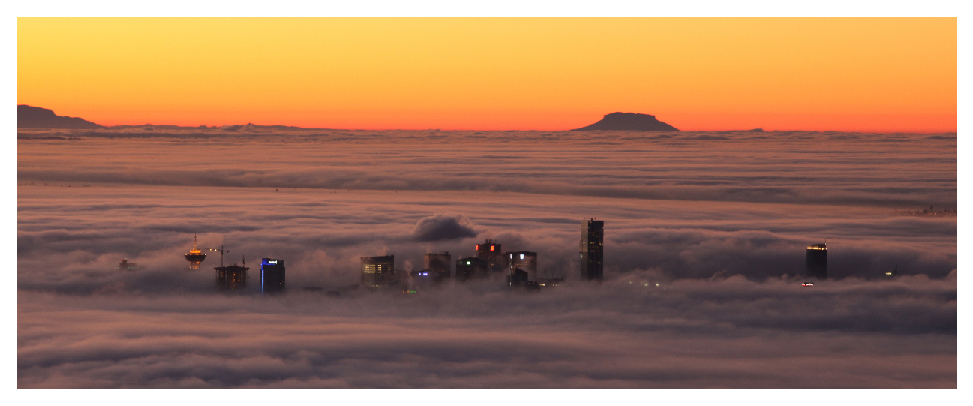
\includegraphics[width=\linewidth]{CypressView}
%   \caption{In the Clouds: Vancouver from Cypress Mountain. Note that the teaser may not be wider than the abstract block.}
%   \label{fig:teaser}
% }

% \begin{teaserfigure}
\teaser{
    \centering
    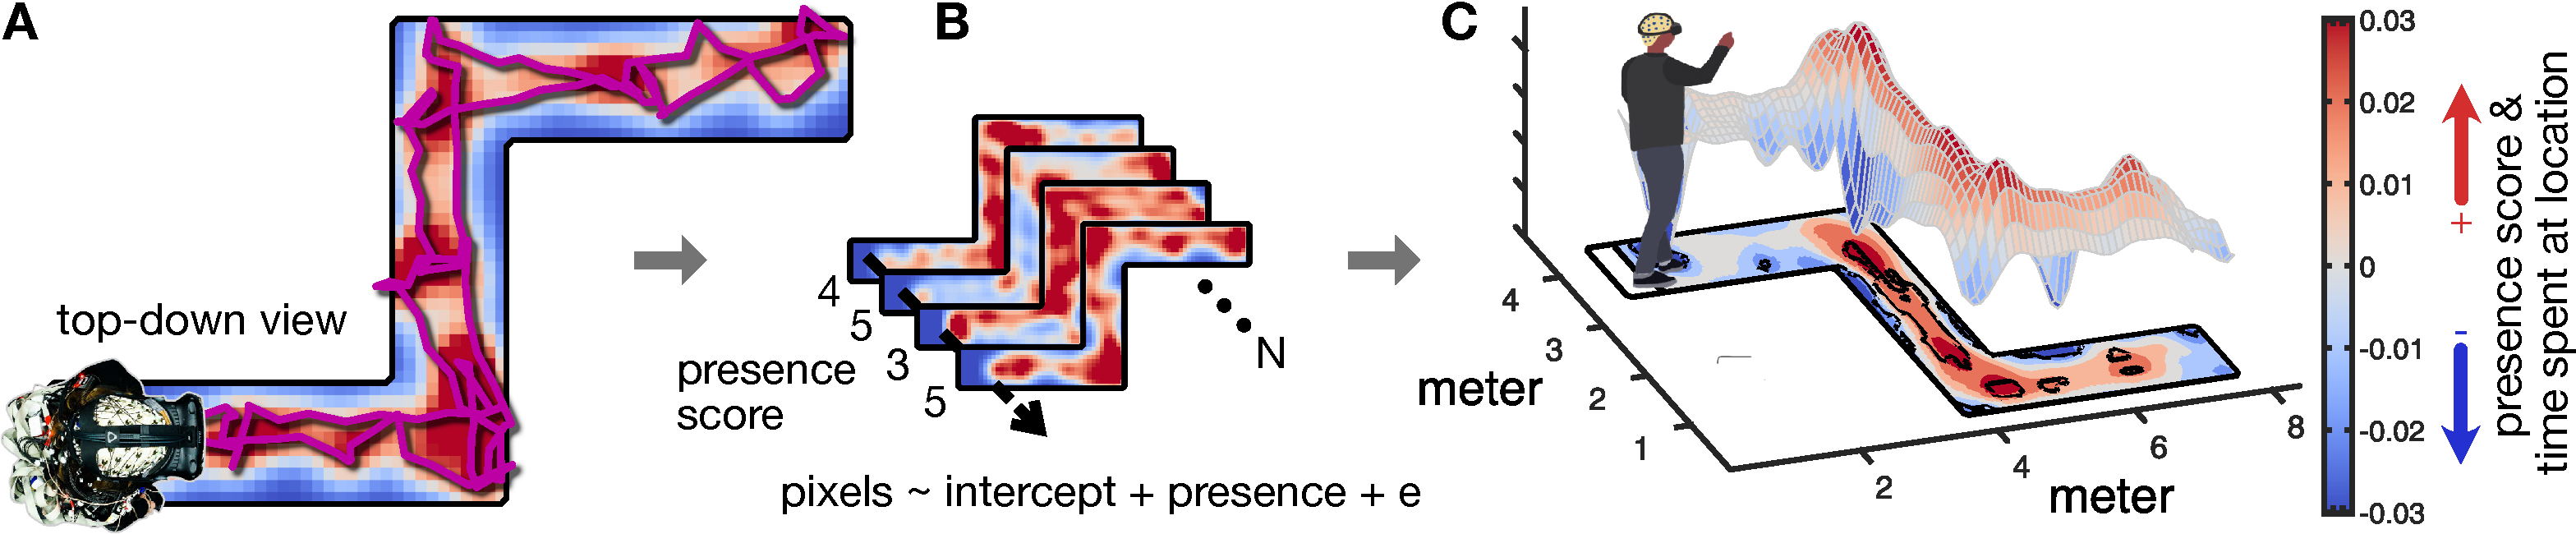
\includegraphics[width=\textwidth]{figures/fig1_3d_new.pdf}
    \caption{We propose parametric maps to study user behavior and experience and guide future design of room-scale VR applications. \textbf{A,} Top-down view on the participant equipped with a wireless VR headset and backpack PC at the start of a `Z' maze. Motion capture of exploration paths (solid pink line) was spatially blurred using a Gaussian filter to obtain images/maps in B suited for across participants analyses of moderating variables. \textbf{B,} We constructed parametric maps of where participants spent time exploring the mazes as a function of their experienced presence. \textbf{C,} We found that with increasing presence, participants were more likely to stay in the center of the paths as well as in segments \textit{presumably} critical for navigational success. Significant pixels at $p<0.05$ are masked with a dotted line}
    % \Description{A: Movement Trajectory of a participant exploring a virtual maze environment. B: Trajectoyies of many participants with their presence questionnaire score given after exploration. C: Regression analyses using presence scores as a predictor variable to express where participants spent time exploring the virtual environment}
    \label{fig:methods}
}
% \end{teaserfigure}

%% Abstract section.
% must be between 150 and 250, so aiming for 200!
\begin{abstract}
The use of head-mounted virtual reality (VR) to induce presence in a computer simulated world has proven to significantly increase the ecological validity of this medium. In VR, illusions of various kinds (place illusion, plausibility illusion, etc.) occur at the same time for the user to feel present. Most prominently, the embodiment illusion has proven to elicit 'realistic' behavioral as well as physiological responses, when a strong emotional stimulus such as virtual hurting of an embodied rubber hand is provided. Yet, to be able to employ VR and claim ecological validity for less emotional stimuli, the level of presence must be accounted for. We show that the level of presence impacts free spatial exploration behavior in a large scale VR navigation paradigm. Here, we investigate the impact of an established presence metric on ongoing motor behavior demonstrating an analysis framework with a high spatial resolution. We observed participants with higher presence to stay closer to the walls while exploring invisible mazes. Ultimately, we link presence to individual differences in video game experience, sex, and spatial perspective taking abilities, confirming that user characteristics are a defining part of the presence construct.
\end{abstract}
% in the end use hemingway app (http://www.hemingwayapp.com) to increase readability
% Word count is 194:
% \abstract{Duis autem vel eum iriure dolor in hendrerit in vulputate
% velit esse molestie consequat, vel illum dolore eu feugiat nulla
% facilisis at vero eros et accumsan et iusto odio dignissim qui blandit
% praesent luptatum zzril delenit augue duis dolore te feugait nulla
% facilisi. Lorem ipsum dolor sit amet, consectetuer adipiscing elit,
% sed diam nonummy nibh euismod tincidunt ut laoreet dolore magna
% aliquam erat volutpat. Ut wisi enim ad minim veniam, quis nostrud exerci tation ullamcorper
% suscipit lobortis nisl ut aliquip ex ea commodo consequat. Duis autem
% vel eum iriure dolor in hendrerit in vulputate velit esse molestie
% consequat, vel illum dolore eu feugiat nulla facilisis at vero eros et
% accumsan et iusto odio dignissim qui blandit praesent luptatum zzril
% delenit augue duis dolore te feugait nulla facilisi.%
% } % end of abstract

%% ACM Computing Classification System (CCS). 
%% See <http://www.acm.org/about/class> for details.
%% We recommend the 2012 system <http://www.acm.org/about/class/class/2012>
%% For the 2012 system use the ``\CCScatTwelve'' which command takes four arguments.
%% The 1998 system <http://www.acm.org/about/class/class/2012> is still possible
%% For the 1998 system use the ``\CCScat'' which command takes four arguments.
%% In both cases the last two arguments (1998) or last three (2012) can be empty.

\CCScatlist{
  \CCScatTwelve{Human-centered computing}{Visu\-al\-iza\-tion}{Visu\-al\-iza\-tion techniques}{Treemaps};
  \CCScatTwelve{Human-centered computing}{Visu\-al\-iza\-tion}{Visualization design and evaluation methods}{}
}

%\CCScatlist{
  %\CCScat{H.5.2}{User Interfaces}{User Interfaces}{Graphical user interfaces (GUI)}{};
  %\CCScat{H.5.m}{Information Interfaces and Presentation}{Miscellaneous}{}{}
%}

%% Copyright space is enabled by default as required by guidelines.
%% It is disabled by the 'review' option or via the following command:
% \nocopyrightspace

%%%%%%%%%%%%%%%%%%%%%%%%%%%%%%%%%%%%%%%%%%%%%%%%%%%%%%%%%%%%%%%%
%%%%%%%%%%%%%%%%%%%%%% START OF THE PAPER %%%%%%%%%%%%%%%%%%%%%%
%%%%%%%%%%%%%%%%%%%%%%%%%%%%%%%%%%%%%%%%%%%%%%%%%%%%%%%%%%%%%%%%%

\begin{document}

%% The ``\maketitle'' command must be the first command after the
%% ``\begin{document}'' command. It prepares and prints the title block.

%% the only exception to this rule is the \firstsection command
\firstsection{Introduction}

\maketitle

% 1 Introduction
% Address the question: What problem are you solving, or opportunity are you seizing? 
\section{1 intro}
Especially in times of a global pandemic, increasing the (psychological) depth of people's remote connections is desirable across the board. Room-scale VR significantly increases the users immersion by, first and foremost, allowing free movements, simulating the sensory \textit{natural} experience in the real world. Further, synchronized motion capture allows avatar movements to be rendered equal to the own bodies movements. In VR, illusions of various kinds (place illusion, plausibility illusion, etc.) occur at the same time for the user to feel present. Depending on the effectiveness of the employed illusions and whether multiple illusions work in congruence, participants experience feeling present in VR \cite{Gonzalez-Franco2017, Kilteni2012}. Most prominently, the embodiment illusion, or body ownership transfer, has proven to elicit \textit{realistic} behavioral as well as physiological responses, when a strong emotional stimulus such as virtual hurting of an embodied rubber hand is provided. Such illusions enrich and/or modify participants subjective experience in VR. Together, free movement, \textit{realisitic} avatar rendering and contextual components of the VR experience coincide at the same time for the user to feel present. Designing immersive experiences for room-scale VR aims at facilitating the emergence of presence experience, dissolving the feeling of connectedness to the real body, ultimately providing the foundation for genuinely connected (social) experiences. 

\section{Zooming in: presence experience and its impact on movement behavior}
In order to scale immersive VR technology to a broader public with use cases ranging from remote office work to entertainment, inclusive design principles are of key importance to successfully designing presence experience across the user base. Individual differences, for example the proclivity to move throughout virtual worlds, significantly challenge designing for presence experience thereby challenging acceptance of VR technology in general \cite{Sagnier2020}. Here, designers and developers would benefit from a rich understanding of user behavior, being able to directly query the impact of certain characteristics of their, unintendedly, neglected user base. Specifically in room-scale VR applications, leveraging inherent motion capture provides the opportunity for data-driven understanding of how individual proclivities explain user experience with spatial specificity. However, typical data reports usually consider aggregate data missing the opportunity to spatially resolve effects of interest.

\begin{figure*}[!ht]
\centering
  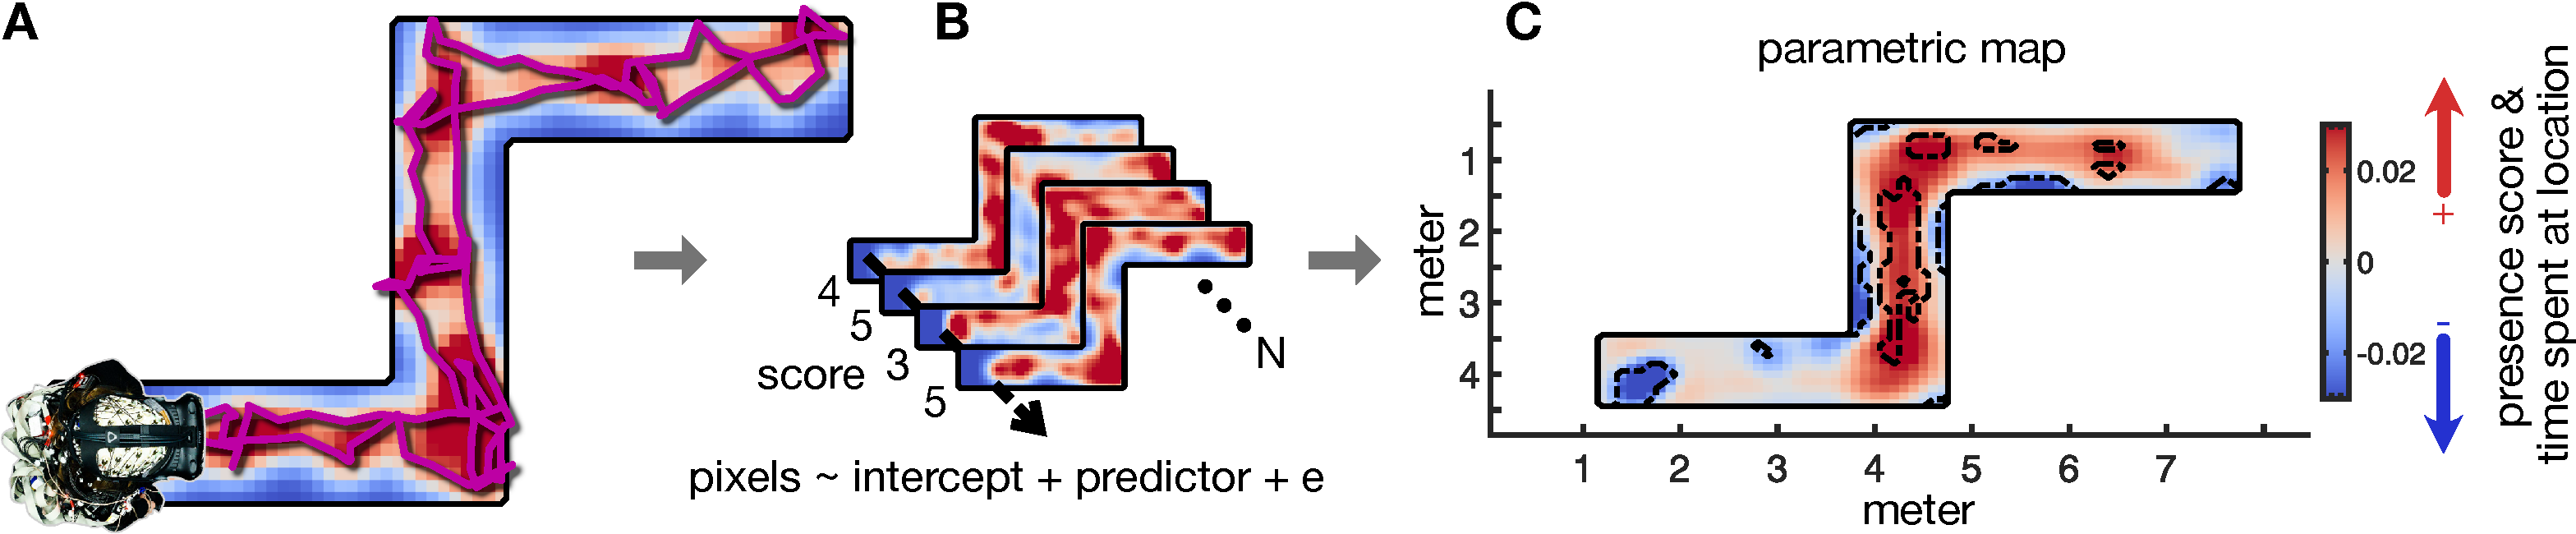
\includegraphics[width=\linewidth]{figures/fig1.pdf}
  %\vspace{-15pt}
  \caption{We propose parametric maps to guide future design decisions of room scale VR applications addressing a broader public. In our study participants explored \textit{invisible} mazes probing hidden walls for visual guidance. \textbf{A:} Motion capture of exploration paths was spatially blurred for across participants analyses of moderating variables. \textbf{B:} We administered experience presence and constructed parametric maps of where participants spent time exploring the mazes as a function of their experienced presence. \textbf{C:} Validating our proposal, we found that with increasing presence, participants were more likely to stay in the center of the paths as well as in segments critical for navigational success.}~\label{fig:methods}
\end{figure*}

We propose using \textit{GLM}, general linear model, in a mass-univariate application across all pixels of a given room-scale VR space. The approach is scalable to many models in the \textit{GLM family} therefore providing a framework with significant flexibility. Further, the analyses scheme is easily extended to 3D space, for example to investigate individual differences in hand reaching scenarios. In this work, we employ the proposed analyses scheme to exhibit how differences in subjectively reported experienced presence impacts participants movement profiles in a \textit{beyond} room-scale VR spatial exploration task. We guide the reader in a step-by-step fashion through the pre-processing, model fitting and inference steps in order to construct spatially resolved \textit{parametric maps}. To highlight potential benefits when considering individual characteristics, we close with a linear regression classification scheme predicting presence via individual characteristics.

%%%%% writing ressources
%As a concurrent effect, we present an easily adaptable and scalable GLM analyses framework to investigate movement behavior with a high spatial resolution.
%Here, we first confirm individual differences in movement profiles of experienced video gamers moving faster and more efficient when exploring a large-scale VR.


% 2 Zooming in (main point) / 3 Related Work
% Address the question: What were the previous solutions to the stated problem?
\section{2 Related Work}
To this day, human development is explainable by the need to interact with a physical reality. Growing up, the human brain \textit{presumably} develops as a model of the latent hidden variables governing the observable behavior of cause and effect in the environment \cite{Friston2010}. Understanding cognition as a predictive process means brains constantly compare what is effectively happening in the world, with what was predicted to happen \cite{Clark2013}, for example inferring the trajectory of a thrown ball and successfully catching it.

\subsection{Natural behavior as a precursor of presence experience}
Successful immersion into virtual worlds relies on matching expectations that were substantiated in the non-virtual physical reality. Assuming that to experience presence in virtual environments equals treating what you perceive as a part of the reality you are currently in, many researchers have argued for an increase in ecological validity through VR experimentation across the cognitive sciences \cite{Bohil2011, Parsons2015, Parsons2017}. The assumption hence is that participants under the influence of successful VR illusions experience presence and therefore behave \textit{realistically} or with higher ecological validity. This work exhibits an approach to quantify such claims with spatial specificity in order to guide future design decisions in research and application. We point out, that this approach is scalable to investigations of spatially resolved behavioral, psychometric and bio-physiological parameters such as controller jerk, hit accuracy for example in video games or electroencephalographic (EEG) parameters \cite{Gehrke2019}.

\subsection{Presence experience impacts behavior}
Generally speaking many studies have investigated participants in VR illusions employing (A) emotionally charged stimulus material or (B) embodiment illusions. Considering (A), \cite{Diemer2015} provide a thorough overview of the intricate interplay between presence and reactions to emotionally charged stimulation in VR. The authors observed a consistently reported link between presence and the emotional experience in VR. They argue, that by varying degrees of arousal, presence impacts psychological as well as physiological responses. Considering (B), we highlight one relevant aspect from the rich literature on the effects of full-body embodiment into avatars \cite{Maister2015}. The proteus effect characterizes behavioral perturbations depending on avatar body attributes. Yee et al. showed that participants being immersed into an 'attractive' avatar moved closer into the interpersonal space of another person \cite{Yee2007}. Further, Banakou et al. demonstrated that within participants, the size of objects was overestimated while embodied into a child body compared to a non-embodied baseline \cite{Banakou2013}. Furthermore, one of the key VR illusions contributing to the subjective construct of presence is the place illusion which can be defined as the perception of oneself being present in a virtual place where one can act, react, and impact the surroundings \cite{Slater2009}. Therefore, self-location, sense of agency, and spatial awareness of the surroundings are strongly impacted by the place illusion and modify behavior \cite{Kilteni2012}. When one perceives oneself in control of ones own actions and observe action consequences in the virtual surroundings, spatial exploration behavior becomes a part of a learning process to adapt motor behavior to the surroundings as opposed to a random chain of actions executed by the user to explore, for instance, only the VR technology itself \cite{Tan2011}. Together, these examples illustrate that presence experience directly impacts cognition, the action-perception cycle.

\subsection{Benefits of studying spatially resolved behavior}
% Summary motivating our work:
% - what is the benefit of spatial resolution?
% find examples of mocap analysis collapsing data to the mean
% - cite studies with interesting findings but not spatially resolved, i.e. grand-averaged
%Problems of prior research in terms of the resolution of behavioral parameters investigate with respect to proteus effect or other. collapsing behavioral parameters to singular events


%%%%% writing resources
%The framework is derived from the neuroscientific methodology of parametric brain imaging, see for example \cite{Friston1994, Pernet2011}.
%mental representation of the surroundings and respectively the motor behavior.
%Novel immersive paradigms in the behavioral cognitive sciences as well as neurosciences subject participants to controlled, yet stimulus rich experiences in head-mounted VR. 
%Therefore, to be able to employ VR and claim ecological validity the level of presence must be accounted for. 

% 4 User Study
\section{User Study}
To demonstrate our proposed method, we investigated whether the level of experienced presence impacts the spatial exploration behavior of participants in a beyond room-scale VR. Here, we used data from a study by Gehrke et al. that uses the \textit{invisible maze task} mimicking a real-world exploration situation such as finding your way in complete darkness~\cite{Gehrke2018, Miyakoshi2021-ni, Gehrke2021-ml}. We conducted the following two-step analysis. First, we constructed parametric maps to assess where participants exploration behavior was impacted as a function of experienced presence. To this end, we investigated fine-grained behavior at each single point in space by conducting mass-univariate pixel-by-pixel modeling of experienced presence on time spent at each location, i.e. pixel. To situate our findings on an individual differences level we followed up with a linear regression scheme, now using aggregated data. We predicted experienced presence using participants characteristics such as video game experience and perspective taking ability (see further details below).

\subsection{Participants, Procedure, Task and Setup} Thirty-two healthy participants (aged 21--45 years, 14 men) participated in the experiment~\cite{Gehrke2018, Gehrke2021-ml}. All participants gave written informed consent to participation and their experimental protocol was approved by the local ethics committee (protocol: GR\_08\_20170428). Three participants were excluded from data analysis due to incomplete data or difficulties in complying with task requirements.

\begin{figure}[!t]
\centering
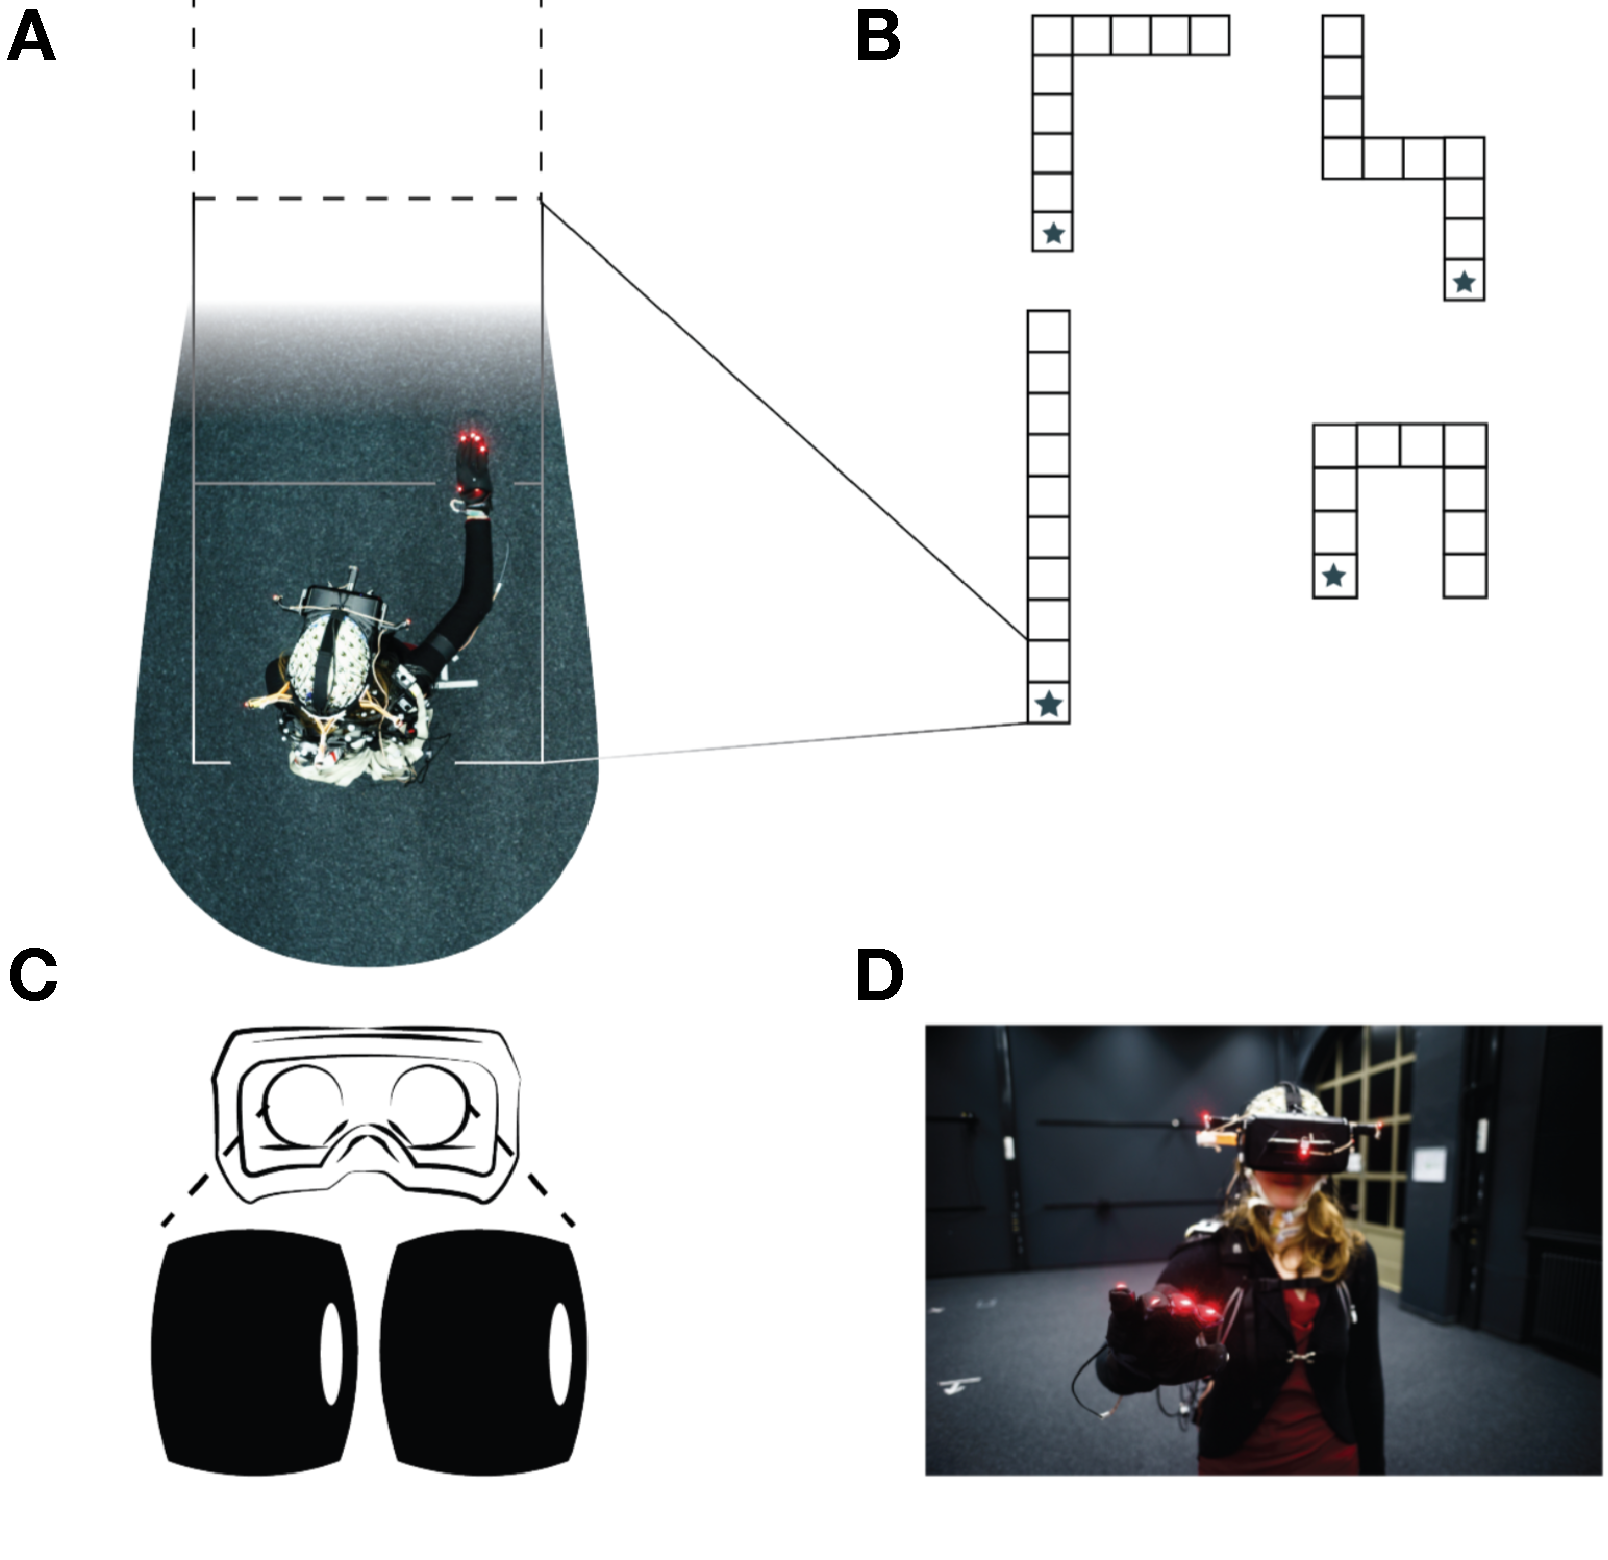
\includegraphics[width=\linewidth]{figures/IMT_Task.pdf}
\vspace{6pt}
\caption{Invisible Maze Task, \textbf{A,} Participant from a bird’s eye view. \textbf{B,} Participants were instructed to explore four different mazes and return to the start.~\cite{Gehrke2018}\textbf{C,} First-person view in binocular `VR optics' of a wall touch. \textbf{D,} Participants were equipped with 160 channels wireless EEG, head-mounted virtual reality goggles and LEDs for motion capture.}
% \Description{A: Top-down view of a participant exploring a virtual maze environment. B: Shapes of the different mazes, shapes are similar to letter I, L, Z and U. C: View inside of the VR headset show a sparse visual feedback occurring when participants touch a wall, much like navigating with a white cane. D: Portrait of a participant during a reach for a wall wearing an EEG Headset and a VR headset.}
\label{imt_task}
\end{figure}

\subsubsection{The Invisible Maze Task} In the experiment participants freely explore a sparse invisible maze environment by walking through virtual mazes and probing for visual feedback when touching the virtual wall of a 1m wide path with their \textit{right} hand. The stimuli were presented using an Oculus Rift DK2 VR headset in combination with a dedicated optical tracking system. Upon collision of the \textit{right} hand with an invisible wall, a white disc appears 30 cm behind the collision point parallel to the invisible wall much like the beam from a torch in a cave, see figure \ref{imt_task} C (consult~\cite{Gehrke2018} for extensive details on the task, instrumentation, and data collection). The left hand was not tracked and participants were instructed to keep the left arm close to their body. Performing the task, participants explored four different mazes in the order, `I', `L', `Z' and `U', see figure \ref{imt_task} B. The task was designed to emphasize participants internal build-up of a spatial representation of the maze layout. Doing the task, participants displayed a behavior that is reported to be comparable to explorative wall touches in the dark to find the way.

For each maze the procedure was as follows: participants were briefly disoriented and then positioned facing the open side of the path. Then, participants were directed to explore the invisible path until they reached a dead end, and subsequently to find their way back to the starting position. At the end of each maze trial, participants received a gamified feedback and were then asked to draw a sketch map of the maze from a bird’s eye view as an index of spatial learning. The procedure was repeated three times in a row for each maze to foster spatial learning. 

The complete experiment, including preparation of physiological measures (Electroencephalogram, EEG) took approximately 4 hours. Preceding and following the task, participants completed a set of questionnaires to assess demographics, spatial abilities, and presence. Synchronized motion capture was collected with behavioral events alongside high-density EEG. For the inquiry in this paper, data of the three exploration phases were aggregated.

\subsubsection{Assessing presence} To assess experienced presence, the igroup presence questionnaire~\cite{Schubert2003} was administered following each individual maze exploration. For our analyses only the first item of the questionnaire was considered, the general subjective presence measure (G1), which represents the sense of being in a place, i.e. `In the computer generated world I had a sense of "being there"' rated from `not at all' to `very much' on a 7-point Likert scale~\cite{Schubert2003, Slater1993}.

%%%%%
%We considered a data-driven approach to finding a useful, i.e. scalable, classification model. Therefore, we initially included a variety of participant descriptors which were subsequently reduced to a set with highest explanatory power. In this way, we progressed towards a minimal model allowing other researchers to reproduce our findings.
\subsection{Statistical Analyses}
With the presented approach we aim to promote benefits of greater spatial resolution of movement behavior to assess a variety of phenomena moderating for example the presence experience in VR. Here, a grand average of, e.g. time spent exploring mazes, provides only limited insights due to its spatial dependence. Some participants may spent more time in the corners but walk faster along straights segments. Without a two-dimensional resolution, this would average out to the same as participants with a constant walking speed. Therefore, we constructed spatial parametric maps. Explained in detail below, we mimicked our approach from established data analyses procedures in cognitive neuroscience and applied it to spatially resolved behavioral data \cite{Friston1994, Bridwell2018a}.

\subsubsection{Parametric Mapping of Ongoing Movement Behavior}
Enabling our proposed analyses framework, two key challenges must be addressed. First, capturing (rigid body) motion in 3D. With state-of-the art VR hardware sampling motion data at around 90Hz accessing and recording the data is possible\footnote{https://brekel.com/openvr-recorder/}. Further libraries to synchronize data streams across the network exist\footnote{See for example https://github.com/sccn/labstreaminglayer and http://openvibe.inria.fr/, with predominant application across the neurosciences.} providing affordable alternatives to dedicated systems.
Second, in order to compare motion data pixel-wise across participants, each participant should exhibit data points at each pixel. Therefore, decreasing spatial resolution by sub-sampling and/or smoothing can be employed to address the challenge.

\textbf{Single-subject summary (a.k.a. first-level).} With this analyses, we were interested in expressing where participants spent most of the time exploring the mazes as a function of experienced presence. To speed up subsequent analyses, we first sub-sampled motion capture data of a rigid body calibrated at the VR Headset, see \ref{imt_task}, to 1Hz. Then we computed individual averages for each maze. We averaged across the three repeated explorations per maze, as we were not interested in changes over time but to express exploration behavior as a function of experienced presence more generally. With an average exploration duration of ~3 minutes, for each maze and participant ~180 samples were kept in x and y, discarding the third dimension (up-down) in this analyses, \ref{imt_task} (left) shows one exploration phase of one subject with lines plotted to connect each sample. 

\textbf{Enabling group-level inference (a.k.a. second-level).} Next, a 2D histogram with fixed edges to maintain equal resolution across participants was computed. In order to increase overlap across participants (second challenge, see above) a 2D (square sized) Gaussian blur was applied to the histogram image. A sigma of 1.5 was chosen for the 2D filter kernel as it resulted in a good overlap across participants while maintaining spatial specificity. 

\textbf{Group-level inference.} To investigate the impact of experienced presence on each parameter, we calculated a linear regression at each pixel of the map. We specified the model as $pixels ~ intercept + presence + error$, hence at each pixel we fit a linear regression across participants with presence scores as the predictor variable. Pixels with data of fewer than 12 participants (critically low N) were kept as `NaN' and not subjected to linear regression analyses. Plotting resulting regression estimates yields a 2D parametric map. Uncorrected p-values were used to plot a contour at significant effects with $p < .05$. The Matlab code used to construct the parametric maps is available online\footnote{}.
% for anonymization: https://github.com/lukasgehrke/mobi-3D-tools

% add GLM toolboxes with resampling

%To address multiple comparison issues with the mass-univariate regression approach, we applied threshold free cluster enhancement to the results F and t maps % cite smith nichols, pernet
%We thresholded the tfce transform of the true result maps at the 95th percentile (alpha $< .05$) of the max tfce distribution of the bootstraps. 
%of interest: first, the time spent at each location as well as the number of wall touches elicited in close proximity. In short, this corresponds to where participants spent most of the time exploring the mazes as well as where they were located when touching the walls most frequently. 

%For the map displaying the number of touches, the 2D histogram count of the location of the participants' head was overwritten by the mean number of touches within the 2D histogram bin

%separately for the two parameters duration and number of touches
\subsubsection{Predicting Presence using Participant Descriptives} 
To follow up our spatially-resolved analyses and situate our findings more generally, we zoomed out and set out to predict presence scores using aggregate data and participant descriptors. We computed a least squares regression entering the IPQ presence (G1) scores as the dependent variable using R~\cite{RFoundationforStatisticalComputing.2018}. To accentuate the effect of aggregating motion capture data we, we included aggregates of movement velocity, time spent exploration or exploration duration. Additionally, we included the average number participants touched a wall with their hand as well as the average accuracy of a sketch map participants had to draw following each exploration. The last metric alludes to an accurate mental spatial representation, which was specifically queried with the \textit{invisible maze task}. We aggregated the measures by computing individual averages over mazes and runs. Further we added participants video game experience, sex, perspective taking and orientation ability and lastly the sense of direction into the regression model. For a detailed explanation of each predictor consult~\cite{Gehrke2018}. Predictors that do not significantly add to the explanatory power of the regression model were localized using a step-wise model selection procedure based on Akaike's information criterion (AIC). The procedure was computed using `stepAIC' of package `MASS'~\cite{Akaike1998a, Venables2002}. This data-driven procedure was selected to exclude the likely problem of over-fitting for the final reported model and to increase the usability of the approach by minimizing the number of included predictors. After the step-wise model selection, three predictors remained in the model predicting presence. Ultimately, the reduced model with three predictors was assessed in terms of its predictive accuracy. Therefore, a 5 fold cross-validation was computed to obtain a robust mean absolute error~\cite{Mosteller1968, Furnkranz2011}. With 29 participants, each training fold consisted of either 23 or 24 participants with either 5 or 6 participants in the evaluated test fold. The R code and data used are available online\footnote{anonymized}.
% for anonymization: https://github.com/lukasgehrke/2019-IEEE-VR-Spatial-exploration-behavior-in-large-scale-VR-predicts-subjective-spatial-presence

% 5 Results
\section{5 results}
We confirmed that the level of experienced presence impacted spatial exploration behavior in VR. Interestingly the effect was similar across different mazes with a pattern of increasing presence associated with staying in the center of the maze path and spending more time in segments \textit{presumably} critical for navigational success. To emphasize the importance to consider individual differences designing room-scale VR for a broad public, we carved out significant individual characteristics predicting the level of experienced presence, potentially of use directing future design decisions.

\begin{figure}[!t]
\centering
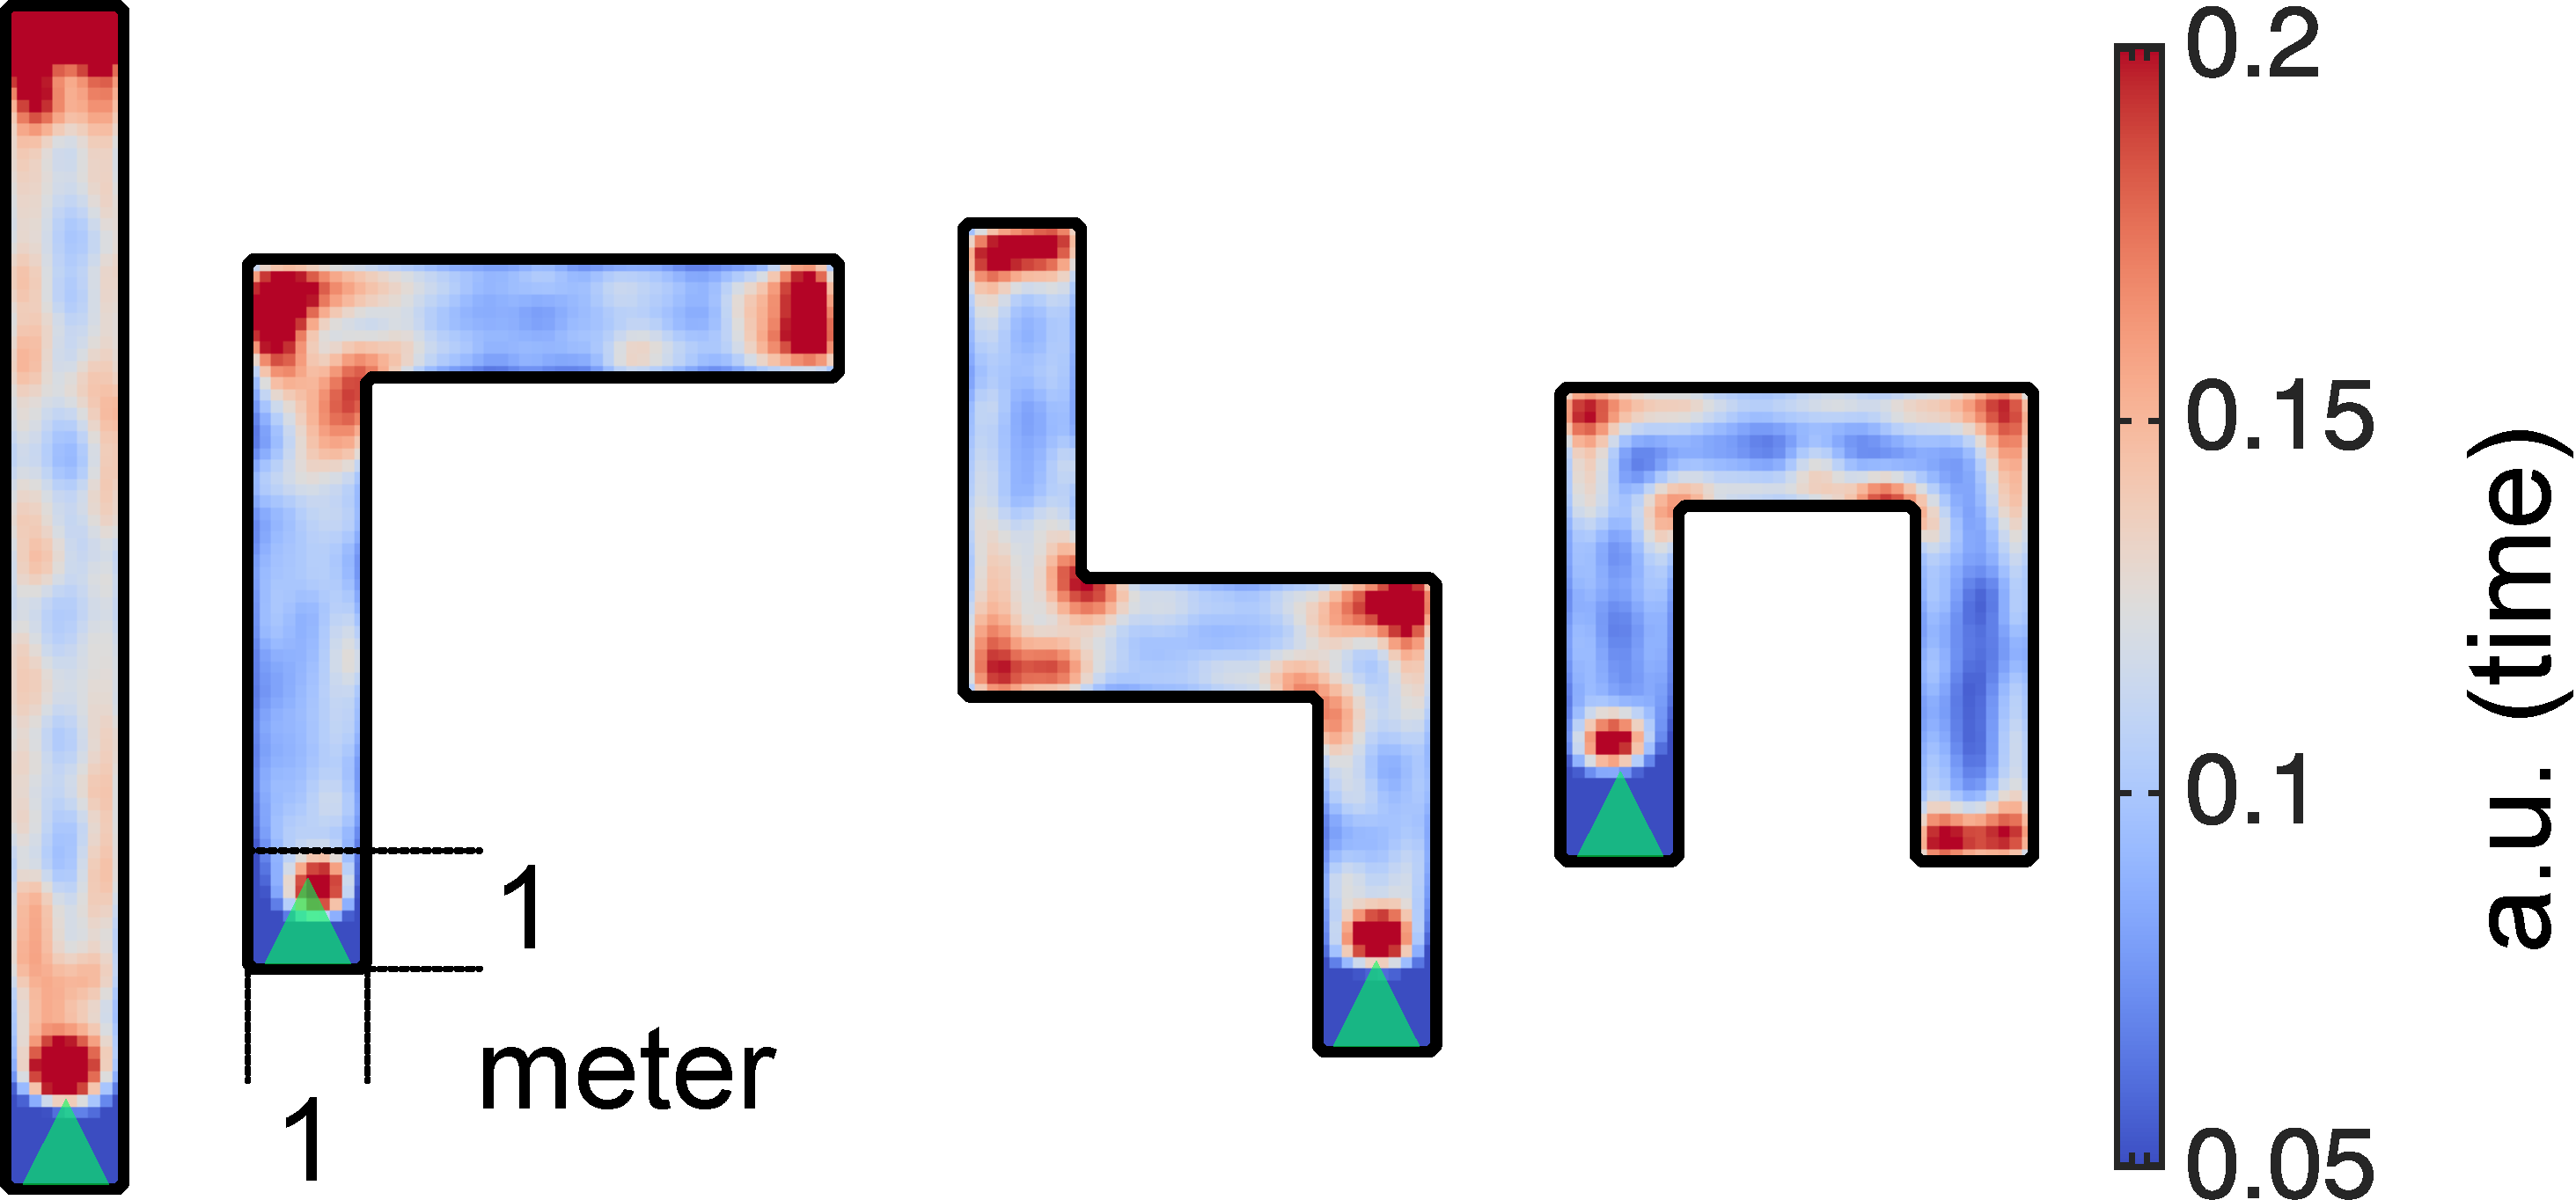
\includegraphics[width=\linewidth]{figures/head_loc_mean2.pdf}
\vspace{6pt}
\caption{Time spent at each location (grand-average) in each of the four mazes: `I', `L', `Z' and `U'. The whole lab space covered roughly 12 by 8 meters in size. Mazes are constructed of ten 1x1 meter squares. Warmer colors, i.e. red, indicate a longer time spent at that location. Green triangles indicate participants starting position.}
\label{head_loc_mean}
\end{figure}
\subsection{Exploration behavior expressed as a function of presence} 
First, averaging spatially-resolved exploration time across participants revealed that participants spent more time in dead-ends as well as in areas including corners. The effect was observed across all mazes (see red colors in figure \ref{head_loc_mean}). Conversely, less time was spent when located in the straight segments of each maze, i.e. participants moved faster in those segments. As expected, participants also spent more time at the beginning of the trial, taking a moment to start moving. Together, these findings confirmed our intuitive expectations of the exploration behavior. 

Second, we investigated the effect of presence on time spent exploring mass-univariately for all locations in all mazes. With increasing presence scores, time spent at the center of the straight paths increased, for example in maze `I' at [3.5, 1.5] $beta=.027, t_{(28)}=2.76, p=.01, R^2=.23$ and `Z' at [1.8, 10] $beta=.039, t_{(28)}=3.34, p<.01, R^2=.34$, see figure \ref{presence_head_loc} A. Further, increasing presence scores correlated with more time spent at the center of the paths in corners, for example in maze `L' at [-1, 3.5] $beta=.037, t_{(28)}=2.33, p=.03, R^2=.19$ and `U' at [0.5, 17.5] $beta=.034, t_{(28)}=2.44, p=.02, R^2=.19$. Conversely, closer to the maze boundaries we observed a negative effect with increasing presence scores correlating with less time spent in these areas, specifically in the most challenging mazes `Z' at [2, 11.5] $beta=-.073, t_{(28)}=-4.16, p<.01, R^2=.40$ and `U' at [0.5, 17] $beta=-.143, t_{(28)}=-4.05 p<.01, R^2=.40$. Taken together, with an increase in experienced presence, participants spent more time firmly located at the center of the path, specifically along the straight segments in the `I' and `Z' maze as well in navigationally relevant corners of mazes `L', `Z' and `U'. Further underlining this observation, higher reported presence scores negatively correlated with the time spent close or even colliding with the maze walls.
\begin{figure}[!h]
\centering
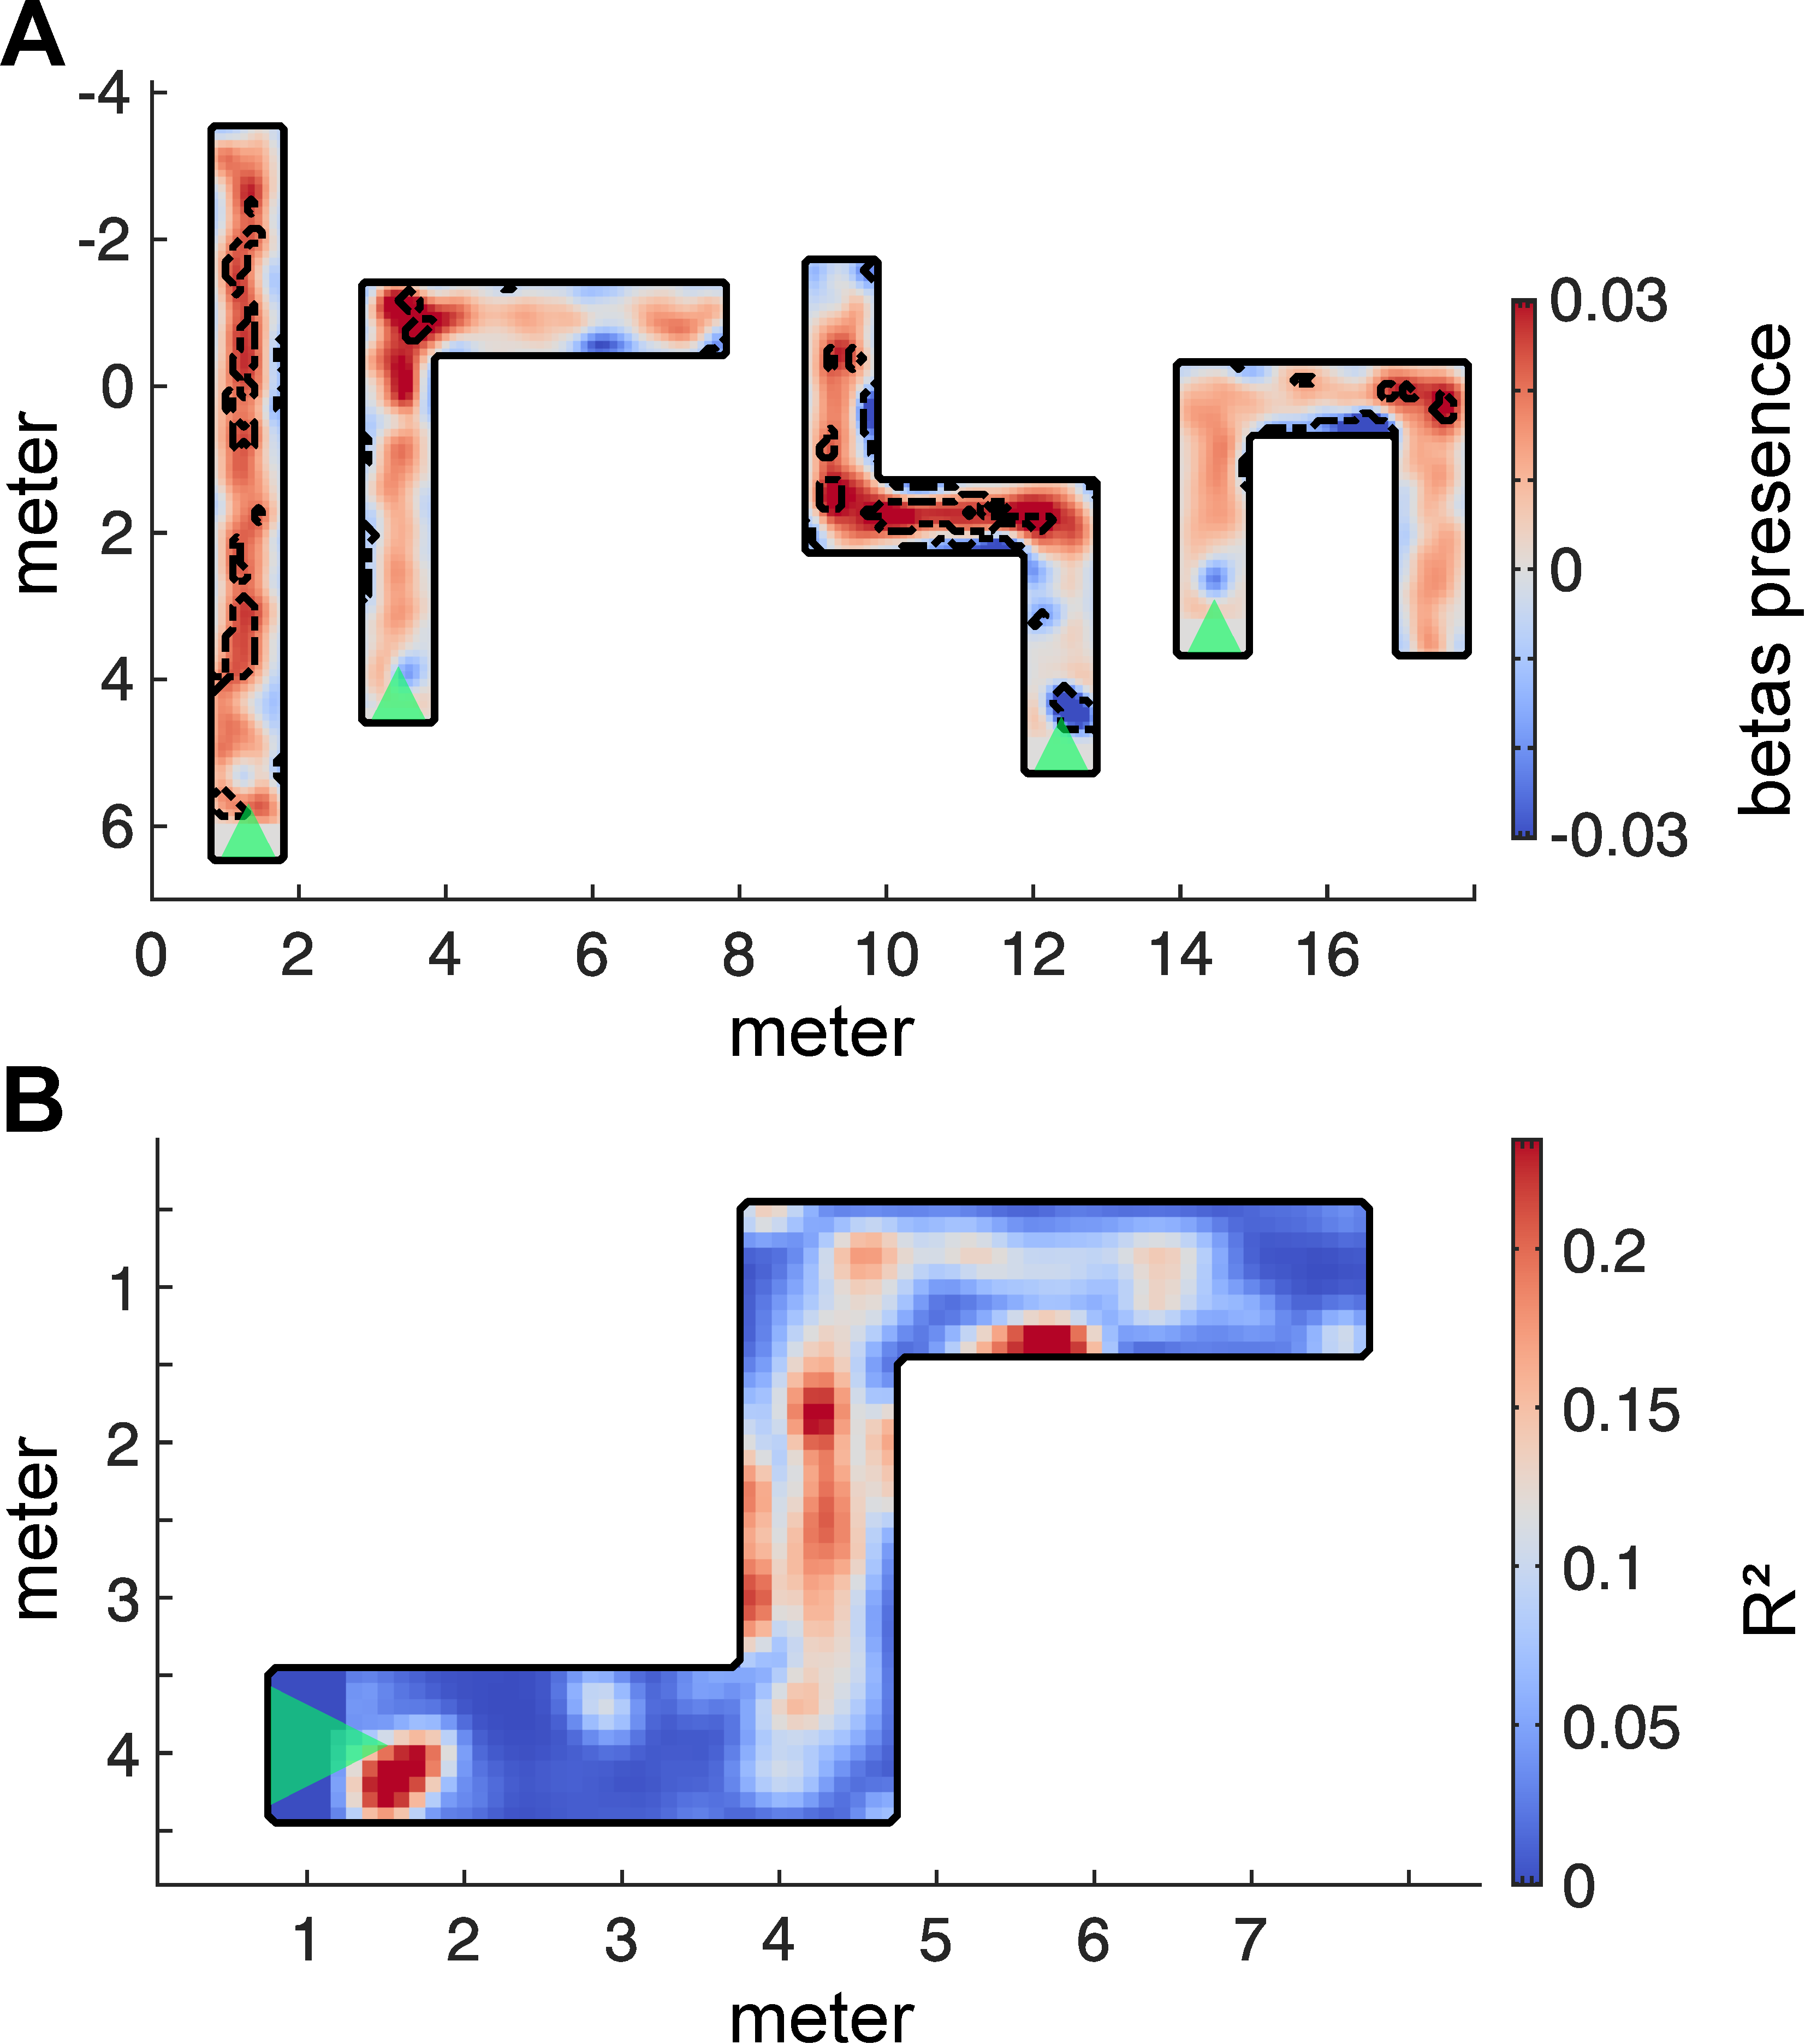
\includegraphics[width=\linewidth]{figures/head_loc_reg2.pdf}
\vspace{6pt}
\caption{Map of the impact of presence on the time spent at every location (betas) in each of the four mazes: `I', `L', `Z', `U'. Green triangles indicate participants starting position. Warmer colors refer to a positive regression estimate. The values can be understood in the sense that for each 1 point increase in reported presence, participants stayed `z' seconds longer at location `xy'. Significant pixels at $p<0.05$ are masked with a dotted line}
\label{presence_head_loc}
\end{figure}

\subsection{Video game experience, biological sex and perspective taking predict presence experience} A step-wise model selection resulted in three remaining predictors, explaining 53,4\% of the variation in experienced presence ($F_{(3,25)}=11.69, p < .001,$ adjusted $R^2=.534$). Participants' predicted presence score was equal to $8.15 - 1.2 (Video Game Experience) + 2.61 (Biological Sex) - 0.02 (PTSOT)$ where biological sex was dummy-coded as 0 = Male, 1 = Female, increasing video game experience was coded with higher scores and decreasing perspective taking ability with higher scores. Video game experience ($t_{(25)}=-4.7, p<.001$), biological  sex ($t_{(25)}=5.6, p<.001$) as well as perspective taking ability ($t_{(25)}=-2.52, p=.02$) were significant predictors of presence. Cross-validation of the three predictor model above yielded a combined average 0.76 mean absolute error. Hence, using video game experience, biological sex as well as perspective taking ability we were able to predict experienced presence with a deviation of $\pm 0.75$ points from the true value on the `IPQ Likert scale'.

% 6 Discussion
\section{6 Contribution, Benefits \& Limitations}
With this paper, we motivate developers and researchers to use parametric mapping using the inherit motion capture capabilities of VR technology for data-driven understanding of user behavior and, ultimately, experience. We introduced parametric maps, expressing VR exploration behavior as a function of experienced presence as an exemplary predictor variable related to the subjective user experience. 

In the user study we showed that increasing subjective presence scores coincided with an increased time spent at the center of the paths' through our simple \textit{invisible} mazes. In turn, this effect translates to participants with high presence scores spending less time closer to the walls, or crashing into them, presumably relating to high spatial awareness. The spatial specificity of our reported effect accentuates that aggregate behavioral metrics, such as average speed or time spent across one maze exploration, may miss critical information. Here a finer resolution has proven to be beneficial.

Our analyses exposed that high presence scores coincided with more time spent in the corners, further underlining the hypotheses of increasing spatial awareness with increasing presence. Sense of embodiment has frequently been included as a key component in psychological models of presence experience with a sense of self-location as one emergence of embodiment~\cite{Kilteni2012}. This sense of a virtual self is a logical prerequisite for spatial anchoring and reduced cognitive effort when imagining a third-person allocentric perspective of space. Here additional mental transformations potentially disrupt the presence experience by violating the \textit{natural} experience of the predictive brain~\cite{Gonzalez-Franco2017}. In consequence, solving spatial task, for example requiring perspective taking, depend on individual abilities and preferences for specific spatial strategies but appear to be `easier' with a congruent sense of embodiment~\cite{Pan2018, Gramann2005, Cognition2016}.

Using participants individual characteristics, we were able to classify presence scores with an average deviation of $/pm 0.75$ from the true reported score. Employing a data-driven model selection procedure determined that apart from video game experience, biological sex as well as perspective taking ability, no other predictor significantly contributed to the linear classification scheme. Interestingly, in our experiment increasing video game experience negatively impacted presence scores, conflicting with previous findings~\cite{Lachlan}. We hypothesize that this could be explained by the overly sparse visuals of the virtual environment in the \textit{invisible maze task}. Participants with significant video gaming experience might perceive the world as too artificial. With regards to the impact of biological sex, we contribute one more example of contradictory results in the literature~\cite{Coluccia2004}. Based on our outcome, however, we cannot argue that the underlying differences in the task were due to a spatial component or rather the interaction with an unknown sparse virtual environment and refer to a detailed discussion on the topic~\cite{Felnhofer}. Ultimately, perspective taking ability had a limited influence predicting subjective presence. Increasing perspective taking scores, referring to an angular error in a mental triangulation task, negatively impacted the subjective feeling of presence. We hypothesize that immersion, as one precursor for the experience of presence may arise earlier in individuals that feel oriented and that are aware of their spatial surroundings. As such, spatial awareness is useful when solving tasks in unfamiliar environments~\cite{Slater2018}.

\section{7 Conclusion}
With this work we motivate continuous, spatially resolved, analyses to understand individual characteristics explaining exploration behavior in VR, ultimately explaining user experience. However, user experience, for example presence experience, is subjective and traditionally assessed via questionnaires following the experience to be evaluated. Such an approach exhibits several advantages. First, a continuous assessment is desirable over a discrete sampling after the VR experience and second, using active and continuous behavioral parameters without interrupting the ongoing experience to administer the questionnaire allows for a non-distorted assessment of presence.

\subsection{Towards an unobtrusive, spatially resolved understanding of user experience}
With this work we showed that observing finely resolved overt behavior may provide hints at the subjective user experience, such as presence experience. Using physiological methods holds the potential to overcome indirect measurement of behavior allowing to directly assess the physiological source that realizes the subjective experience, i.e. the brain~\cite{Gehrke2019, Singh2018, Si-mohammed2020}. Gehrke et al. demonstrated that neural responses associated with mental error-processing following visuo-haptic mismatches in VR can be detected using EEG~\cite{Gehrke2019}. Recently, Si-Mohammed et al. were able to use this EEG signature in a brain-computer interface classification scheme exhibiting high classification accuracy in a similar paradigm exhibiting graphical glitches in VR. These promising findings, hint at future applications in room-scale scenarios, picking up scenarios where a loss of immersion occurs in near real-time. Here, additional wearable sensors can supplement brain recordings to, for example, measure affective responses~\cite{Marin-Morales2018}.

To sum up, we propose a method to investigate user experience in VR by using a spatially resolved analyses approach of ongoing behavior, providing designers and researchers a tool to guide future design decisions. Investigating how individual characteristics and the current spatial context influences user experience provides the opportunity for inclusive design decisions driving VR technology acceptance across the broad public. Ultimately, we believe our approach can further be nurtured by unobtrusive, continuous (neuro-)physiological measurements for a multi-dimensional assessment of user experience.

% %% \section{Introduction} %for journal use above \firstsection{..} instead
% This template is for papers of VGTC-sponsored conferences which are \emph{\textbf{not}} published in a special issue of TVCG.

% \section{Using the Style Template}

% \begin{itemize}
% \item If you receive compilation errors along the lines of ``\texttt{Package ifpdf Error: Name clash, \textbackslash ifpdf is already defined}'' then please add a new line ``\texttt{\textbackslash let\textbackslash ifpdf\textbackslash relax}'' right after the ``\texttt{\textbackslash documentclass[journal]\{vgtc\}}'' call. Note that your error is due to packages you use that define ``\texttt{\textbackslash ifpdf}'' which is obsolete (the result is that \texttt{\textbackslash ifpdf} is defined twice); these packages should be changed to use ifpdf package instead.
% \item The style uses the hyperref package, thus turns references into internal links. We thus recommend to make use of the ``\texttt{\textbackslash autoref\{reference\}}'' call (instead of ``\texttt{Figure\~{}\textbackslash ref\{reference\}}'' or similar) since ``\texttt{\textbackslash autoref\{reference\}}'' turns the entire reference into an internal link, not just the number. Examples: \autoref{fig:sample} and \autoref{tab:vis_papers}.
% \item The style automatically looks for image files with the correct extension (eps for regular \LaTeX; pdf, png, and jpg for pdf\LaTeX), in a set of given subfolders (figures/, pictures/, images/). It is thus sufficient to use ``\texttt{\textbackslash includegraphics\{CypressView\}}'' (instead of ``\texttt{\textbackslash includegraphics\{pictures/CypressView.jpg\}}'').
% \item For adding hyperlinks and DOIs to the list of references, you can use ``\texttt{\textbackslash bibliographystyle\{abbrv-doi-hyperref-narrow\}}'' (instead of ``\texttt{\textbackslash bibliographystyle\{abbrv\}}''). It uses the doi and url fields in a bib\TeX\ entry and turns the entire reference into a link, giving priority to the doi. The doi can be entered with or without the ``\texttt{http://dx.doi.org/}'' url part. See the examples in the bib\TeX\ file and the bibliography at the end of this template.\\[1em]
% \textbf{Note 1:} occasionally (for some \LaTeX\ distributions) this hyper-linked bib\TeX\ style may lead to \textbf{compilation errors} (``\texttt{pdfendlink ended up in different nesting level ...}'') if a reference entry is broken across two pages (due to a bug in hyperref). In this case make sure you have the latest version of the hyperref package (i.\,e., update your \LaTeX\ installation/packages) or, alternatively, revert back to ``\texttt{\textbackslash bibliographystyle\{abbrv-doi-narrow\}}'' (at the expense of removing hyperlinks from the bibliography) and try ``\texttt{\textbackslash bibliographystyle\{abbrv-doi-hyperref-narrow\}}'' again after some more editing.\\[1em]
% \textbf{Note 2:} the ``\texttt{-narrow}'' versions of the bibliography style use the font ``PTSansNarrow-TLF'' for typesetting the DOIs in a compact way. This font needs to be available on your \LaTeX\ system. It is part of the \href{https://www.ctan.org/pkg/paratype}{``paratype'' package}, and many distributions (such as MikTeX) have it automatically installed. If you do not have this package yet and want to use a ``\texttt{-narrow}'' bibliography style then use your \LaTeX\ system's package installer to add it. If this is not possible you can also revert to the respective bibliography styles without the ``\texttt{-narrow}'' in the file name.\\[1em]
% DVI-based processes to compile the template apparently cannot handle the different font so, by default, the template file uses the \texttt{abbrv-doi} bibliography style but the compiled PDF shows you the effect of the \texttt{abbrv-doi-hyperref-narrow} style.
% \end{itemize}

% \section{Bibliography Instructions}

% \begin{itemize}
% \item Sort all bibliographic entries alphabetically but the last name of the first author. This \LaTeX/bib\TeX\ template takes care of this sorting automatically.
% \item Merge multiple references into one; e.\,g., use \cite{Max:1995:OMF,Kitware:2003} (not \cite{Kitware:2003}\cite{Max:1995:OMF}). Within each set of multiple references, the references should be sorted in ascending order. This \LaTeX/bib\TeX\ template takes care of both the merging and the sorting automatically.
% \item Verify all data obtained from digital libraries, even ACM's DL and IEEE Xplore  etc.\ are sometimes wrong or incomplete.
% \item Do not trust bibliographic data from other services such as Mendeley.com, Google Scholar, or similar; these are even more likely to be incorrect or incomplete.
% \item Articles in journal---items to include:
%   \begin{itemize}
%   \item author names
% 	\item title
% 	\item journal name
% 	\item year
% 	\item volume
% 	\item number
% 	\item month of publication as variable name (i.\,e., \{jan\} for January, etc.; month ranges using \{jan \#\{/\}\# feb\} or \{jan \#\{-{}-\}\# feb\})
%   \end{itemize}
% \item use journal names in proper style: correct: ``IEEE Transactions on Visualization and Computer Graphics'', incorrect: ``Visualization and Computer Graphics, IEEE Transactions on''
% \item Papers in proceedings---items to include:
%   \begin{itemize}
%   \item author names
% 	\item title
% 	\item abbreviated proceedings name: e.\,g., ``Proc.\textbackslash{} CONF\_ACRONYNM'' without the year; example: ``Proc.\textbackslash{} CHI'', ``Proc.\textbackslash{} 3DUI'', ``Proc.\textbackslash{} Eurographics'', ``Proc.\textbackslash{} EuroVis''
% 	\item year
% 	\item publisher
% 	\item town with country of publisher (the town can be abbreviated for well-known towns such as New York or Berlin)
%   \end{itemize}
% \item article/paper title convention: refrain from using curly brackets, except for acronyms/proper names/words following dashes/question marks etc.; example:
% \begin{itemize}
% 	\item paper ``Marching Cubes: A High Resolution 3D Surface Construction Algorithm''
% 	\item should be entered as ``\{M\}arching \{C\}ubes: A High Resolution \{3D\} Surface Construction Algorithm'' or  ``\{M\}arching \{C\}ubes: A high resolution \{3D\} surface construction algorithm''
% 	\item will be typeset as ``Marching Cubes: A high resolution 3D surface construction algorithm''
% \end{itemize}
% \item for all entries
% \begin{itemize}
% 	\item DOI can be entered in the DOI field as plain DOI number or as DOI url; alternative: a url in the URL field
% 	\item provide full page ranges AA-{}-BB
% \end{itemize}
% \item when citing references, do not use the reference as a sentence object; e.\,g., wrong: ``In \cite{Lorensen:1987:MCA} the authors describe \dots'', correct: ``Lorensen and Cline \cite{Lorensen:1987:MCA} describe \dots''
% \end{itemize}

% \section{Example Section}

% Lorem\marginpar{\small You can use the margins for comments while editing the submission, but please remove the marginpar comments for submission.} ipsum dolor sit amet, consetetur sadipscing elitr, sed diam
% nonumy eirmod tempor invidunt ut labore et dolore magna aliquyam erat,
% sed diam voluptua. At vero eos et accusam et justo duo dolores et ea
% rebum. Stet clita kasd gubergren, no sea takimata sanctus est Lorem
% ipsum dolor sit amet. Lorem ipsum dolor sit amet, consetetur
% sadipscing elitr, sed diam nonumy eirmod tempor invidunt ut labore et
% dolore magna aliquyam erat, sed diam
% voluptua~\cite{Kitware:2003,Max:1995:OMF}. At vero eos et accusam et
% justo duo dolores et ea rebum. Stet clita kasd gubergren, no sea
% takimata sanctus est Lorem ipsum dolor sit amet. Lorem ipsum dolor sit
% amet, consetetur sadipscing elitr, sed diam nonumy eirmod tempor
% invidunt ut labore et dolore magna aliquyam erat, sed diam
% voluptua. At vero eos et accusam et justo duo dolores et ea
% rebum. Stet clita kasd gubergren, no sea takimata sanctus est.

% \section{Exposition}

% Duis autem vel eum iriure dolor in hendrerit in vulputate velit esse
% molestie consequat, vel illum dolore eu feugiat nulla facilisis at
% vero eros et accumsan et iusto odio dignissim qui blandit praesent
% luptatum zzril delenit augue duis dolore te feugait nulla
% facilisi. Lorem ipsum dolor sit amet, consectetuer adipiscing elit,
% sed diam nonummy nibh euismod tincidunt ut laoreet dolore magna
% aliquam erat volutpat~\cite{Kindlmann:1999:SAG}.

% \begin{equation}
% \sum_{j=1}^{z} j = \frac{z(z+1)}{2}
% \end{equation}

% Lorem ipsum dolor sit amet, consetetur sadipscing elitr, sed diam
% nonumy eirmod tempor invidunt ut labore et dolore magna aliquyam erat,
% sed diam voluptua. At vero eos et accusam et justo duo dolores et ea
% rebum. Stet clita kasd gubergren, no sea takimata sanctus est Lorem
% ipsum dolor sit amet. Lorem ipsum dolor sit amet, consetetur
% sadipscing elitr, sed diam nonumy eirmod tempor invidunt ut labore et
% dolore magna aliquyam erat, sed diam voluptua. At vero eos et accusam
% et justo duo dolores et ea rebum. Stet clita kasd gubergren, no sea
% takimata sanctus est Lorem ipsum dolor sit amet.

% \subsection{Lorem ipsum}

% Lorem ipsum dolor sit amet (see \autoref{tab:vis_papers}), consetetur sadipscing elitr, sed diam
% nonumy eirmod tempor invidunt ut labore et dolore magna aliquyam erat,
% sed diam voluptua. At vero eos et accusam et justo duo dolores et ea
% rebum. Stet clita kasd gubergren, no sea takimata sanctus est Lorem
% ipsum dolor sit amet. Lorem ipsum dolor sit amet, consetetur
% sadipscing elitr, sed diam nonumy eirmod tempor invidunt ut labore et
% dolore magna aliquyam erat, sed diam voluptua. At vero eos et accusam
% et justo duo dolores et ea rebum. Stet clita kasd gubergren, no sea
% takimata sanctus est Lorem ipsum dolor sit amet. Lorem ipsum dolor sit
% amet, consetetur sadipscing elitr, sed diam nonumy eirmod tempor
% invidunt ut labore et dolore magna aliquyam erat, sed diam
% voluptua. At vero eos et accusam et justo duo dolores et ea
% rebum. 

% \begin{table}[tb]
%   \caption{VIS/VisWeek accepted/presented papers: 1990--2016.}
%   \label{tab:vis_papers}
%   \scriptsize%
% 	\centering%
%   \begin{tabu}{%
% 	r%
% 	*{7}{c}%
% 	*{2}{r}%
% 	}
%   \toprule
%    year & \rotatebox{90}{Vis/SciVis} &   \rotatebox{90}{SciVis conf} &   \rotatebox{90}{InfoVis} &   \rotatebox{90}{VAST} &   \rotatebox{90}{VAST conf} &   \rotatebox{90}{TVCG @ VIS} &   \rotatebox{90}{CG\&A @ VIS} &   \rotatebox{90}{VIS/VisWeek} \rotatebox{90}{incl. TVCG/CG\&A}   &   \rotatebox{90}{VIS/VisWeek} \rotatebox{90}{w/o TVCG/CG\&A}   \\
%   \midrule
% 	2016 & 30 &   & 37 & 33 & 15 & 23 & 10 & 148 & 115 \\
%   2015 & 33 & 9 & 38 & 33 & 14 & 17 & 15 & 159 & 127 \\
%   2014 & 34 &   & 45 & 33 & 21 & 20 &   & 153 & 133 \\
%   2013 & 31 &   & 38 & 32 &   & 20 &   & 121 & 101 \\
%   2012 & 42 &   & 44 & 30 &   & 23 &   & 139 & 116 \\
%   2011 & 49 &   & 44 & 26 &   & 20 &   & 139 & 119 \\
%   2010 & 48 &   & 35 & 26 &   &   &   & 109 & 109 \\
%   2009 & 54 &   & 37 & 26 &   &   &   & 117 & 117 \\
%   2008 & 50 &   & 28 & 21 &   &   &   & 99 & 99 \\
%   2007 & 56 &   & 27 & 24 &   &   &   & 107 & 107 \\
%   2006 & 63 &   & 24 & 26 &   &   &   & 113 & 113 \\
%   2005 & 88 &   & 31 &   &   &   &   & 119 & 119 \\
%   2004 & 70 &   & 27 &   &   &   &   & 97 & 97 \\
%   2003 & 74 &   & 29 &   &   &   &   & 103 & 103 \\
%   2002 & 78 &   & 23 &   &   &   &   & 101 & 101 \\
%   2001 & 74 &   & 22 &   &   &   &   & 96 & 96 \\
%   2000 & 73 &   & 20 &   &   &   &   & 93 & 93 \\
%   1999 & 69 &   & 19 &   &   &   &   & 88 & 88 \\
%   1998 & 72 &   & 18 &   &   &   &   & 90 & 90 \\
%   1997 & 72 &   & 16 &   &   &   &   & 88 & 88 \\
%   1996 & 65 &   & 12 &   &   &   &   & 77 & 77 \\
%   1995 & 56 &   & 18 &   &   &   &   & 74 & 74 \\
%   1994 & 53 &   &   &   &   &   &   & 53 & 53 \\
%   1993 & 55 &   &   &   &   &   &   & 55 & 55 \\
%   1992 & 53 &   &   &   &   &   &   & 53 & 53 \\
%   1991 & 50 &   &   &   &   &   &   & 50 & 50 \\
%   1990 & 53 &   &   &   &   &   &   & 53 & 53 \\
%   \midrule
%   \textbf{sum} & \textbf{1545} & \textbf{9} & \textbf{632} & \textbf{310} & \textbf{50} & \textbf{123} & \textbf{25} & \textbf{2694} & \textbf{2546} \\
%   \bottomrule
%   \end{tabu}%
% \end{table}

% \subsection{Mezcal Head}

% Lorem ipsum dolor sit amet (see \autoref{fig:sample}), consetetur sadipscing elitr, sed diam
% nonumy eirmod tempor invidunt ut labore et dolore magna aliquyam erat,
% sed diam voluptua. At vero eos et accusam et justo duo dolores et ea
% rebum. Stet clita kasd gubergren, no sea takimata sanctus est Lorem
% ipsum dolor sit amet. Lorem ipsum dolor sit amet, consetetur
% sadipscing elitr, sed diam nonumy eirmod tempor invidunt ut labore et
% dolore magna aliquyam erat, sed diam voluptua. At vero eos et accusam
% et justo duo dolores et ea rebum. Stet clita kasd gubergren, no sea
% takimata sanctus est Lorem ipsum dolor sit amet. 

% \subsubsection{Duis Autem}

% Lorem ipsum dolor sit amet, consetetur sadipscing elitr, sed diam
% nonumy eirmod tempor invidunt ut labore et dolore magna aliquyam erat,
% sed diam voluptua. At vero eos et accusam et justo duo dolores et ea
% rebum. Stet clita kasd gubergren, no sea takimata sanctus est Lorem
% ipsum dolor sit amet. Lorem ipsum dolor sit amet, consetetur
% sadipscing elitr, sed diam nonumy eirmod tempor invidunt ut labore et
% dolore magna aliquyam erat, sed diam voluptua. At vero eos et accusam
% et justo duo dolores et ea rebum. Stet clita kasd gubergren, no sea
% takimata sanctus est Lorem ipsum dolor sit amet. Lorem ipsum dolor sit
% amet, consetetur sadipscing elitr, sed diam nonumy eirmod tempor
% invidunt ut labore et dolore magna aliquyam erat, sed diam
% voluptua. At vero eos et accusam et justo duo dolores et ea
% rebum. Stet clita kasd gubergren, no sea takimata sanctus est. Lorem
% ipsum dolor sit amet.

% \begin{figure}[tb]
%  \centering % avoid the use of \begin{center}...\end{center} and use \centering instead (more compact)
%  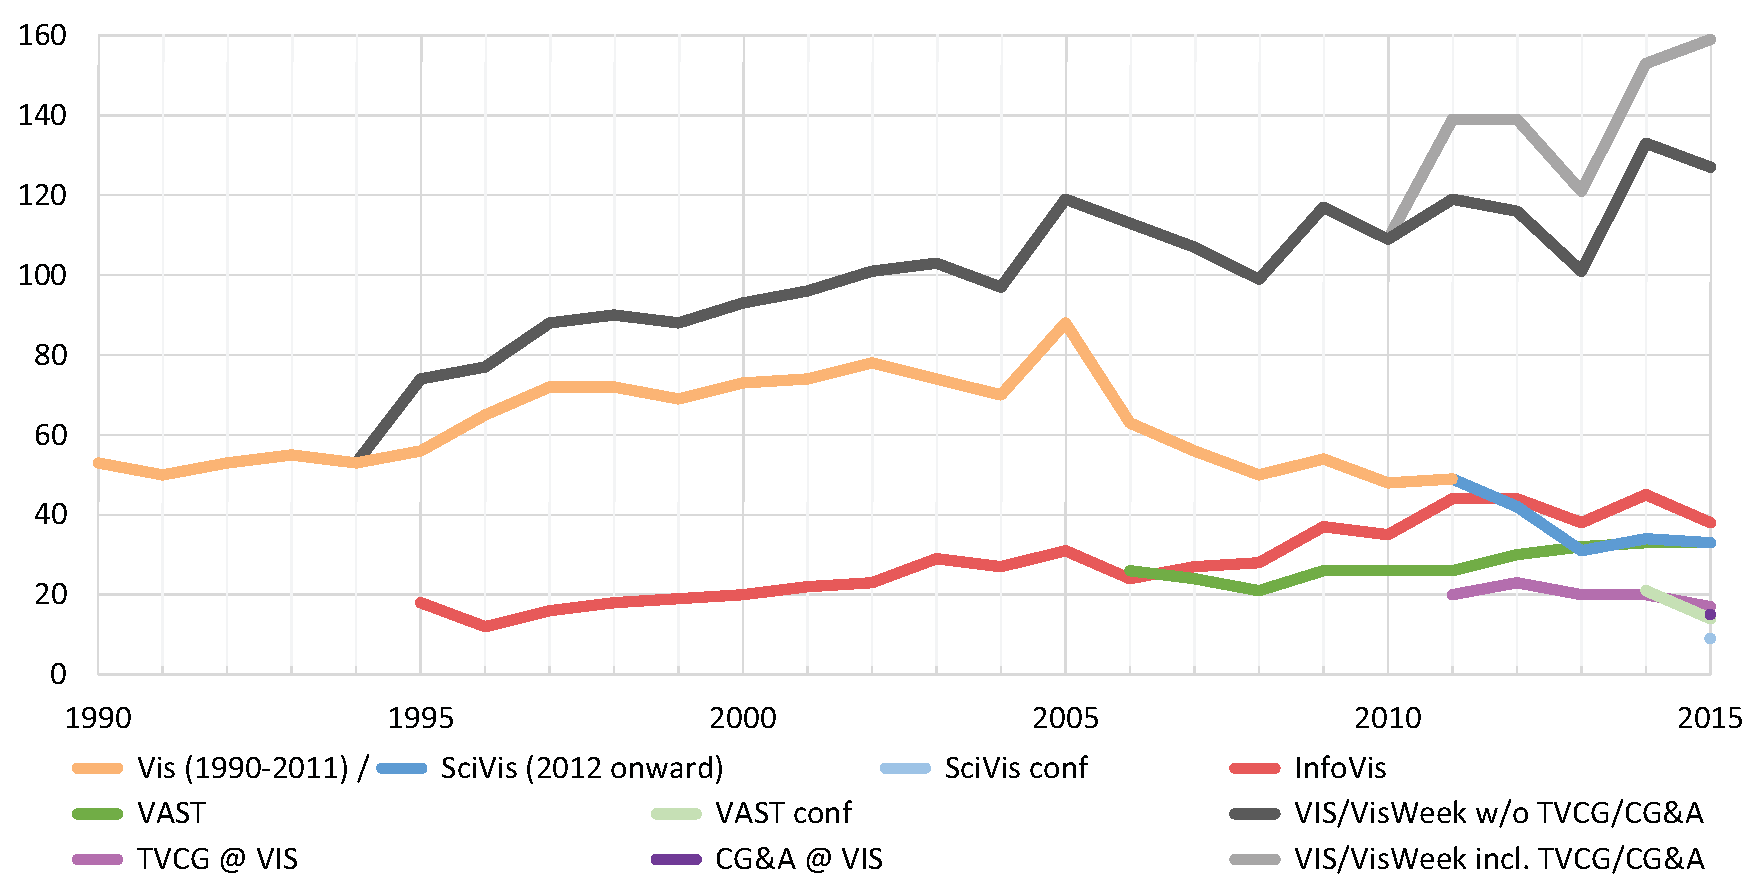
\includegraphics[width=\columnwidth]{paper-count-w-2015-new}
%  \caption{A visualization of the 1990--2015 data from \autoref{tab:vis_papers}. The image is from \cite{Isenberg:2017:VMC} and is in the public domain.}
%  \label{fig:sample}
% \end{figure}

% \subsubsection{Ejector Seat Reservation}

% Duis autem~\cite{Lorensen:1987:MCA}\footnote{The algorithm behind
% Marching Cubes \cite{Lorensen:1987:MCA} had already been
% described by Wyvill et al. \cite{Wyvill:1986:DSS} a year
% earlier.} vel eum iriure dolor in hendrerit
% in vulputate velit esse molestie consequat,\footnote{Footnotes
% appear at the bottom of the column.} vel illum dolore eu
% feugiat nulla facilisis at vero eros et accumsan et iusto odio
% dignissim qui blandit praesent luptatum zzril delenit augue duis
% dolore te feugait nulla facilisi. Lorem ipsum dolor sit amet,
% consectetuer adipiscing elit, sed diam nonummy nibh euismod tincidunt
% ut laoreet dolore magna aliquam erat volutpat.


% \paragraph{Confirmed Ejector Seat Reservation}

% Ut wisi enim ad minim veniam, quis nostrud exerci tation ullamcorper
% suscipit lobortis nisl ut aliquip ex ea commodo
% consequat~\cite{Nielson:1991:TAD}. Duis autem vel eum iriure dolor in
% hendrerit in vulputate velit esse molestie consequat, vel illum dolore
% eu feugiat nulla facilisis at vero eros et accumsan et iusto odio
% dignissim qui blandit praesent luptatum zzril delenit augue duis
% dolore te feugait nulla facilisi.

% \paragraph{Rejected Ejector Seat Reservation}

% Ut wisi enim ad minim veniam, quis nostrud exerci tation ullamcorper
% suscipit lobortis nisl ut aliquip ex ea commodo consequat. Duis autem
% vel eum iriure dolor in hendrerit in vulputate velit esse molestie


% \section{Conclusion}

% Lorem ipsum dolor sit amet, consetetur sadipscing elitr, sed diam
% nonumy eirmod tempor invidunt ut labore et dolore magna aliquyam erat,
% sed diam voluptua. At vero eos et accusam et justo duo dolores et ea
% rebum. Stet clita kasd gubergren, no sea takimata sanctus est Lorem
% ipsum dolor sit amet. Lorem ipsum dolor sit amet, consetetur
% sadipscing elitr, sed diam nonumy eirmod tempor invidunt ut labore et
% dolore magna aliquyam erat, sed diam voluptua. At vero eos et accusam
% et justo duo dolores et ea rebum. Stet clita kasd gubergren, no sea
% takimata sanctus est Lorem ipsum dolor sit amet. Lorem ipsum dolor sit
% amet, consetetur sadipscing elitr, sed diam nonumy eirmod tempor
% invidunt ut labore et dolore magna aliquyam erat, sed diam
% voluptua. At vero eos et accusam et justo duo dolores et ea
% rebum.


%% if specified like this the section will be committed in review mode
%\acknowledgments{
%Some ideas for this work developed during an internship at Chatham Labs %(acquired by Facebook) under the guidance of Mark Parent.
%}

%\bibliographystyle{abbrv}
\bibliographystyle{abbrv-doi}
%\bibliographystyle{abbrv-doi-narrow}
%\bibliographystyle{abbrv-doi-hyperref}
%\bibliographystyle{abbrv-doi-hyperref-narrow}

% \bibliography{template}
\bibliography{bibliography}
\end{document}
